\chapter{Conclusion}
\section{Project Summary}

Over the course of the project, the Kinect development landscape has changed dramatically as more and more academics and companies are recognising the benefit of the range imaging technology behind the Kinect. This has led to several changes in the underlying software for the Kinect which our project has had to adapt to during this time. The project is now an established `proof of concept' for the determination of volume and limb circumference using range imaging technologies. It is also a platform for performing markerless recognition for ultrasound scanners who require repeated scans of a specific area of the body. From our initial discussions with our project supervisor and from the original concept as specified by Paul Summers and Massimo Pelligrini, the group has managed to deliver a system which satisfies this functionality to a reasonably accurate degree. Given the novel nature of this project, we feel that the literature emerging in the area regarding the applications of range imaging in this area have not been fully explored and thus gives plenty of opportunity for extension and refinement. \\

\section{Further Work}
This section details the potential further work that could be undertaken.\\

\subsection{Evolving SDKs}
While this project was being completed other toolkits and SDKs have been released to provide the means to access and manipulate data from range sensors, such as the Kinect. As the project was nearing its completion and deadline, Microsoft released version 1.7 of their SDK which included built-in registration support known as \emph{Kinect Fusion}. Experimentation showed that the Kinect Fusion component was not capable of registering human objects but it would be interesting to experiment with various parameters and see if this is at all possible. If registration were successful then the results could be compared and contrasted to see who's approach made the best trade-offs between efficiency and accuracy.   

\subsection{3D Image Acquisition Pipeline}
The registration methods could have benefited from being supplied with simple objects of known quantities for testing purposes. This was, unfortunately, not possible due to a rigidly implemented object isolation algorithm further up the pipeline which only allowed human objects to be scanned in, using the Kinect's skeleton tracking APIs. \\

This issue was partially rectified by measuring so called \emph{gold standards} for certain individuals using the Archimedes method for body volume calculation. In the future, a parallel pipeline could be created to allow arbitrary objects to be scanned in or a module could be developed to import scan data from outside the programme. \\

\subsection{3D Rendering}
As mentioned in the evaluation of our functional requirements (Section \ref{eval:functional}), the rendering of 3D models is not currently produced in real time. In the future this could be improved upon through the implementation of some 3D rendering library, such as OpenGL or by sampling the point cloud for rendering, as the visualisation currently exists primarily for aesthetic reasons. \\

\section{Volume Estimation}
This section details how further work would improve the accuracy of the volume estimation.\\

\subsection{Transform Constant}
\label{transform constant}
Due to time constraints, the constant used to transform between point cloud space and real world space is only valid under a specific set of circumstances. Specifically, the patient must be 2.2m away from the Kinect, the Kinect must be 71cm off the ground and the Kinect's elevation must be 0, as stated in Section \ref{test strategy}. Such conditions may be too restrictive in a doctor's surgery. Given more time and considerably more data, a function of distance $d$, height of camera $h_c$ and the angle of the camera $\theta$ could be derived to determine the best fitting transform constant, rather than a one size fits all approach as is currently used. The patients height $h_p$ could also be incorporated into this function, as in Figure \ref{a potential transform function}.\\

\begin{figure}[h]
    \begin{center}
      $Transform Constant = f(d,h_c,\theta,h_p)$
    \end{center}
    \caption{A potential transform function}
    \label{a potential transform function}
\end{figure}

\subsection{Concave Hulls}
A plane used for volume calculation is passed to the convex hull algorithm before having its circumference calculated. A convex hull over estimates the circumference, especially around the legs. Such an effect is due to the figure of 8 shape of a leg plane. A better hull algorithm would be a concave hull \cite{moreira2007}. However a limitation of concave hulls is that they are not unique, see Figure \ref{multiple valid concave hulls}, therefore this limitation must be overcome before it can be included in the project.\\

\begin{figure}[h]
\begin{center}
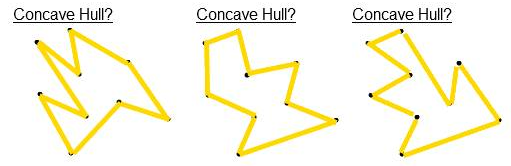
\includegraphics[scale=0.6]{images/concave}
\end{center}
\caption{Multiple valid concave hulls}
\label{multiple valid concave hulls}
\end{figure}


\subsection{General}
As mentioned above in Section \ref{transform constant}, the main item required is more data. Due to the difficulty and potential embarrassment of measuring a person volume through a bath tub, only three people had a gold standard for volume measurement. More gold standards would allow for more reliable conclusions to be drawn about the accuracy of the volume estimation.\\

\section{Limb Circumference}

Limb circumference is limited by the inaccuracies of mapping skeletal data to point cloud space and hence also suffers from the noise inherent in the low resolution depth data received by the Kinect. A more robust limb circumference mechanism that exploited real-time reconstruction would have produced point clouds with finer detail and hence a more accurate circumference measurement from the selected limbs. A method that was cited in the Design section regarding the fitting of ellipses to cross sections of the body could also be explored but from empirical evidence cited by the authors, this was shown to suffer from large degrees of error due to the noise present in the Kinect data.

\susection{Markerless Recognition}
One of the main limitations of the project is the requirement that no new or modified hardware be required. This changes the dynamic of the sensor tracking problem in particular, limiting it to an image processing problem. Were additional or modified hardware available, there would be a great number of different ways to solve the problem with greater ease than image processing. For example, having additional positioning hardware inside the sensor could provide 3D tracking with much greater ease than via optics.\\

Although impressive given the time available, the tracking of the sensor is very shaky and not particularly reliable. There are measures which could improve performance, but the main constraints are image quality and lighting. For improved accuracy, higher resolution imagery is required, and of better quality. The Kinect does provide a higher resolution 1280x720 feed at 12fps, but it is interpolated information rather than from its native resolution which reduces its quality yet further in terms of colour reproduction and spacial accuracy. The combination of the Kinect with a full HD sensor could provide significantly better tracking, with a spacial resolution nearer 2mm per pixel.\\

Control over lighting and the materials used to provide the green colouring would help significantly as the colour detected across the sensor would vary much less, allowing a more constrained colour search.\\

Given the time and scope to improve the stability of the depth feed, both the tracking and the scanning sections of the project could be greatly advanced. To foray deep into three-dimensional feature and search algorithms would be most insightful, though significantly more complex.\\
